\pdfoutput=1
\documentclass[a0,portrait,25pt]{sciposter}

% Служи за оформяне на текста в колони.
\usepackage{multicol}

% Задава разстоянието между колоните в постера.
\columnsep=20pt

% Задава дебелината на линията разделяща колоните в постера.
\columnseprule=1pt

% Задава цветове според техните SVG названия. Пълният списък с цветовете е наличен на: http://www.latextemplates.com/svgnames-colors
\usepackage[svgnames]{xcolor}

% Използване на Times шрифтовете.
\usepackage{times}

% Използва се за включването на изображения.
\usepackage{graphicx}
\graphicspath{{images/}}

% Позволява промяна на фоновия цвят. 
\usepackage{pagecolor}

% Позволява използването на текст в кутии и фонов цвят.
\usepackage{mdframed}

\begin{document}

% Фонов цвят на постера.
\pagecolor{LightGray}

\begin{mdframed}[backgroundcolor=white,roundcorner=4pt,shadow=true,linewidth=1pt]
\begin{minipage}[b]{1.44  \linewidth}
\begin{multicols}{2}
\
\color{DimGray}
\Huge \textbf{Multilayer Perceptron Training \\ Randomized by Second Instance of \\ Multilayer Perceptron} \\
% Имена на авторите.
\huge {Todor Balabanov, Iliyan Zankinski, Kolyu Kolev} \\ [0.5cm] 
% Название на института.
\huge Institute of Information and Communication Technologies \\  Bulgarian Academy of Sciences \\ [0.4cm]
% Електронен адрес за връзка.
\Large \texttt{todorb@iinf.bas.bg}


\includegraphics[width=20cm]{logo-iict-en}
\end{multicols}
\end{minipage}
\end{mdframed}

% Разстояние между заглавната част на постера и същинското изложение. 
\vspace{0.5cm}

% Въведение. 
\begin{mdframed}[backgroundcolor=white,roundcorner=4pt,shadow=true,linewidth=1pt]
\color{Black}
\section*{Introduction}
Multilayer perceptron is one of the most used types of artificial neural network. For the last four decades artificial neural networks are heavily researched and used in real industrial solutions [1,2]. The power of artificial neural networks is in their operating phase. Once trained artificial neural networks are an extremely efficient tool [3]. The training phase of the artificial neural network is the problematic part of their usage. Training is usually too slow and not always efficient enough. Multilayer perceptron is weighted directed graph organized in layers. When multilayer perceptron is fully connected each neuron from a single layer is connected with each neuron from the next layer. Neurons are the nodes in the graph where links between nodes are weighted. The calculating power of multilayer perceptron is in its weights. Finding proper values for the weights is a global optimization problem. Each neuron collects signals as its input. Signals are coming from other neurons or from external for the multilayer perceptron environment. Signals are multiplied by the weight of the link and then their sum is calculated. The sum of the weighted signals is usually normalized by the activation function of each neuron. Such normalization is a key feature of the multilayer perceptron, because the number of neuron's input links is variable and there is no limitation of the weights range. The most used activation functions are the hyperbolic tangent and the sigmoid function.  In the literature there are hundreds training algorithms, but the most popular and the most used one is the back-propagation training. Back-propagation is exact numerical method and it is based on the gradient of the multilayer perceptron output error. Speed-up of multilayer perceptron training is always desirable and this study proposes usage of second multilayer perceptron which randomizes the back-propagation training procedure of the basic multilayer perceptron. 
\end{mdframed}

% Разделя постера в три колони.
\begin{multicols}{3}

% Обяснение какво представлява обучението с обратно разпространение на грешката.
\begin{mdframed}[backgroundcolor=white,roundcorner=4pt,shadow=true,linewidth=1pt]
\color{Black}
\section*{Back-propagation Training}
\begin{minipage}[c]{1\linewidth}
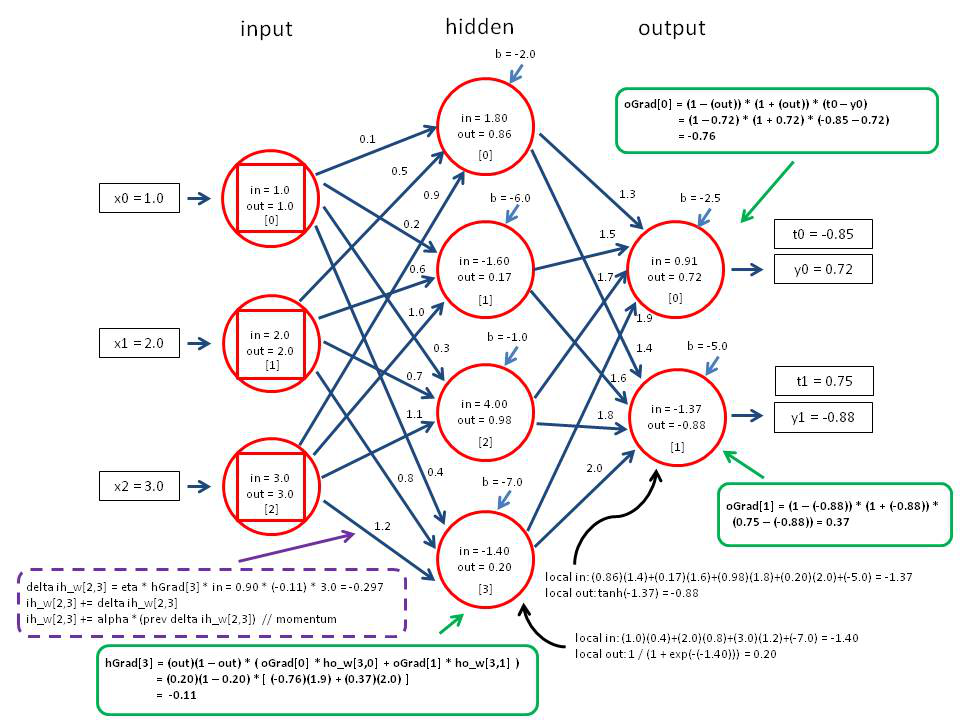
\includegraphics[width=0.9\linewidth]{fig01}
\end{minipage}
https://jamesmccaffrey.files.wordpress.com\\/2012/11/backpropagationcalculations.jpg
\end{mdframed}

% Схема на изкуствен неврон..
\begin{mdframed}[backgroundcolor=white,roundcorner=4pt,shadow=true,linewidth=1pt]
\color{Black}
\section*{Artificial Neuron}
\begin{minipage}[c]{1\linewidth}
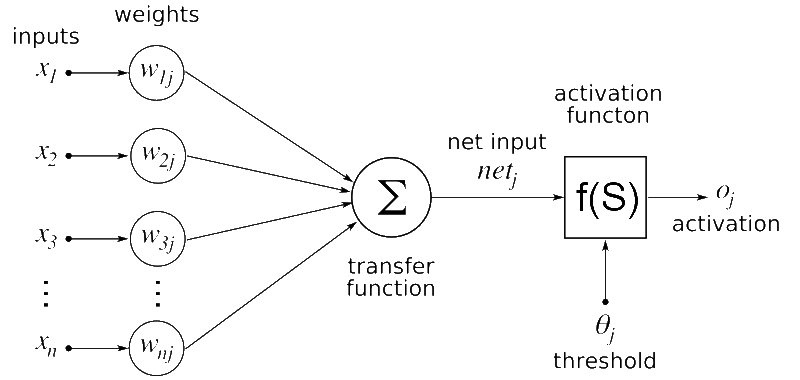
\includegraphics[width=0.9\linewidth]{fig03}
\end{minipage}
https://upload.wikimedia.org/wikipedia\\/commons/b/b6/Artificial\_neural\_network.png
\end{mdframed}

% Обяснение какво представлява случайното прехвърляне на сигнали между две изкуствени невронни мрежи.
\begin{mdframed}[backgroundcolor=white,roundcorner=4pt,shadow=true,linewidth=1pt]
\color{Black}
\section*{Randomization with Second MLP}
\end{mdframed}

% Представяне на хиперболичния тангенс и сигмоидната функция.
\begin{mdframed}[backgroundcolor=white,roundcorner=4pt,shadow=true,linewidth=1pt]
\color{Black}
\section*{Hyperbolic Tangent and Sigmoid Function}
\begin{minipage}[c]{1\linewidth}
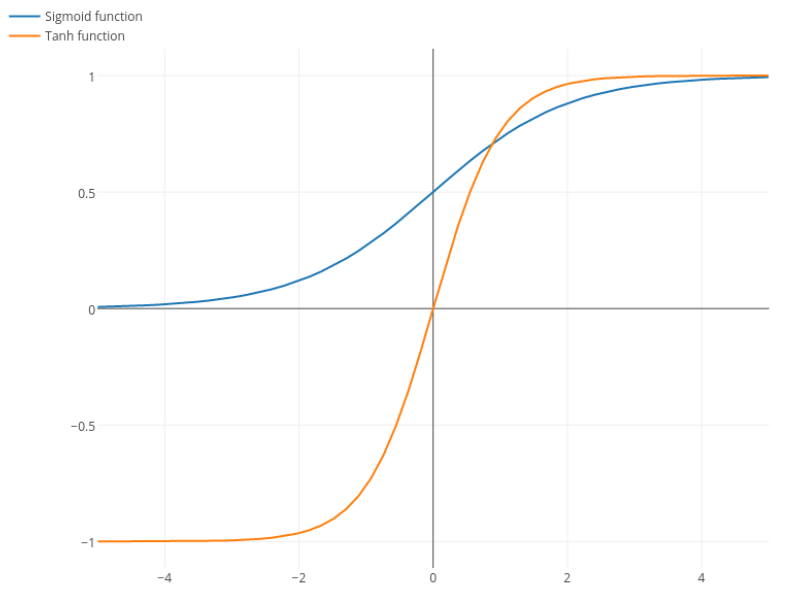
\includegraphics[width=0.9\linewidth]{fig02}
\end{minipage}
https://i.stack.imgur.com/o0JA0.png
\end{mdframed}

% Представяне на проведените експерименти.
\begin{mdframed}[backgroundcolor=white,roundcorner=4pt,shadow=true,linewidth=1pt]
\color{Black}
\section*{Experiments}
\begin{itemize}
\item Both MLPs implemented in Encog for Java
\item Common topology 255-266-10
\item First configuration
\begin{itemize}
  \item Primary MLP with hyperbolic tangent
  \item Secondary MPL with hyperbolic tangent
\end{itemize}
\item Second configuration
\begin{itemize}
  \item Primary MLP with hyperbolic tangent
  \item Secondary MPL with sigmoid function
\end{itemize}
\item Resilient propagation learning algorithm
\item Optical character recognition of digits
\item Weights migration rate of 1\%
\item Independent runs - 30
\end{itemize}
\end{mdframed}

% Представяне на получените резултати.
\begin{mdframed}[backgroundcolor=white,roundcorner=4pt,shadow=true,linewidth=1pt]
\color{Black}
\section*{Results}
\begin{minipage}[c]{1\linewidth}
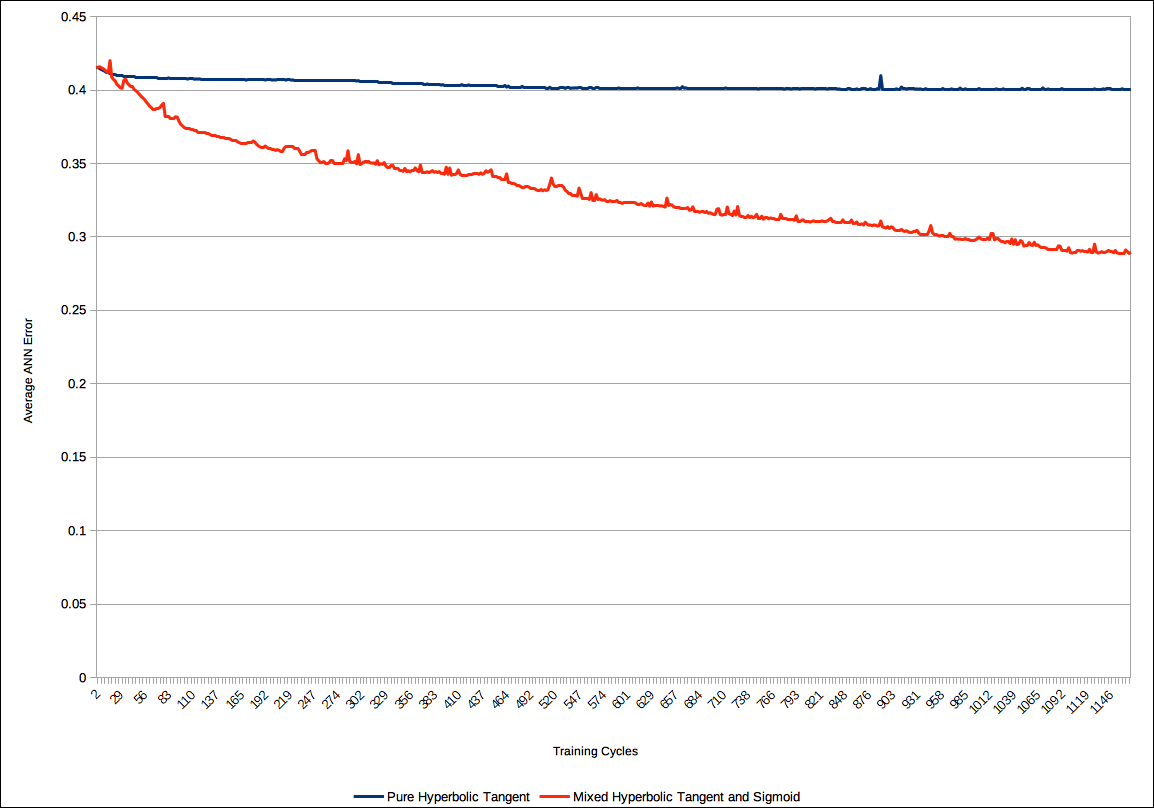
\includegraphics[width=0.9\linewidth]{fig04}
\end{minipage}
\end{mdframed}

% Обощение за извършените изследвания и получените резултати.
\begin{mdframed}[backgroundcolor=white,roundcorner=4pt,shadow=true,linewidth=1pt]
\color{Black}
\section*{Conclustions}
All initial experiments are done with open source software solution, based on Encog Machine Learning Framework ( https://www.heatonresearch.com/encog/ ). Randomization of the weights in the basic multilayer perceptron lead to stairs like convergence curve. As parallel to the neutral neural networks, such stress on the neurons is observed when the neural cells are overloaded and their performance is sensitively reduced. The proposed back-propagation training modification is very promising if it is used in hybrid implementations. As further work it will be interesting if more than two different activation functions are used. 
\end{mdframed}

% Секция за служебна информация.
\begin{mdframed}[backgroundcolor=white,roundcorner=4pt,shadow=true,linewidth=1pt]
\color{Black}
% Биглиография.
\section*{References}
\begin{enumerate}
\item Atanasova, T., Barova, M., Balabanov, T., \textit{Using neural models to analyze time series in large volumes of data}, International Conference  NVU “Vasil Levski”, 193--198, ISSN:1314-1937, (2016) 
\item Tomov, P., Monov, V., \textit{Artificial Neural Networks and Differential Evolution Used for Time Series Forecasting in Distributed Environment}, Proceedings of International conference Automatics and Informatics, ISSN 1313-1850, 129--132, Sofia, Bulgaria, (2016) 
\item Tashev, T., Hristov, H., Modeling of synthesis of information processes with generalized nets. In: Drinov, M. (ed.) Cybernetics and Information Technologies, vol. 2, Academic Publishing House, Sofia, 92–104, (2003) 
\end{enumerate}
\end{mdframed}

% Благодарности.
\begin{mdframed}[backgroundcolor=white,roundcorner=4pt,shadow=true,linewidth=1pt]
\section*{Acknowledgements}
This work was supported by a private funding of Velbazhd Software LLC. 


\includegraphics[width=0.98\linewidth]{veld_soft_camp_fire_logo}
\end{mdframed}
\end{multicols}

% Информация за конференцията. 
\begin{mdframed}[backgroundcolor=white,roundcorner=4pt,shadow=true,linewidth=1pt]
\color{Black}
13th Annual Meeting of the Bulgarian Section of SIAM, December 18 - 20, 2018, Sofia, Bulgaria
\end{mdframed}

\end{document}
